% Copyright 2011 by Frank Wood

\documentclass{beamer}
\usepackage{algorithm}
\usepackage{algorithmic}
\usepackage{natbib}

% Setup appearance:

\usetheme{Darmstadt}
%\usetheme{Copenhagen}
\usefonttheme[onlylarge]{structurebold}
\setbeamerfont*{frametitle}{size=\normalsize,series=\bfseries}
\setbeamertemplate{navigation symbols}{}

% Standard packages
\usepackage[english]{babel}
%\usepackage[latin1]{inputenc}
%\usepackage{times}
%\usepackage[T1]{fontenc}
%\usepackage{nnfootnote}
\usepackage{amsfonts}
\usepackage{amsmath}
%\newcommand{\argmax}{\operatornamewithlimits{argmax}}
\def\newblock{\hskip .11em plus .33em minus .07em}
% Setup TikZ

%\usepackage{tikz}
%\usetikzlibrary{arrows}
%\tikzstyle{block}=[draw opacity=0.7,line width=1.4cm]


% Author, Title, etc.

\title[An Introduction to the Dirichlet Process and Nonparametric Bayesian Models] 
{
	An Introduction to the Dirichlet Process and Nonparametric Bayesian Models
}

\author[Pfau]
{
  Frank~Wood %\inst{1}
}

\institute[Columbia University]
{
  %\inst{1}%
  Columbia University
}

\date[26 April 2010]
{26 Apr 2010}

%\def\blfootnote{\xdef\@thefnmark{}\@footnotetext}

% The main document

\begin{document}

\begin{frame}
	\titlepage
\end{frame}

\section{Introduction}
\subsection{Motivation}

\begin{frame}
\frametitle{Spike Sorting}
\only<1>{
\begin{block}{Spike Sorting Schematic}
	\begin{center}
			\begin{figure}
			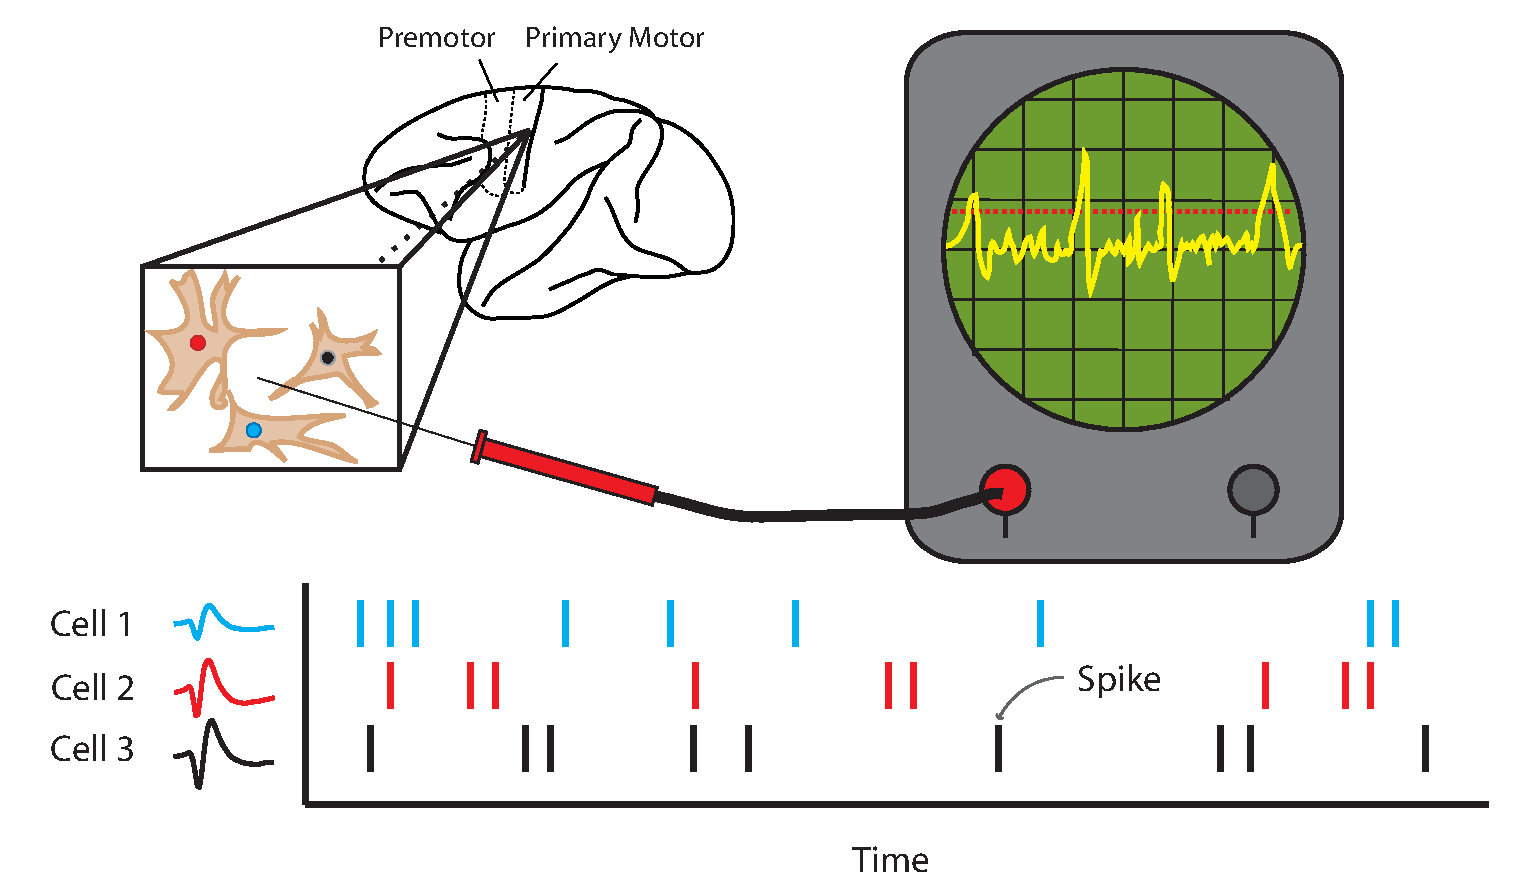
\includegraphics[width=90mm]{figures/spike_sorting_schematic.pdf}
			\caption{\footnotesize Illustration of spike train acquisition}
			%\caption{\footnotesize Brain schematic from \cite{aflalog06}}
			\end{figure}
			\end{center}
			\end{block}
}
\only<2-3>{
\begin{block}{Steps}
\begin{enumerate}
\item{Eliminate noise}
\item{Detect action potentials}
%	\begin{itemize}
%	\item Manual: template matching, thresholding
%	\end{itemize}
\item{Deconvolve overlapping action potentials}
%	\begin{itemize}
%	\item Manual: painstakingly analyze or discard ambiguous data
%	\end{itemize}
	\alert<3>\item{Identify the number of neurons in the recording}
	\alert<3>\item{Attribute spikes to neurons}
	\item{Track changes in action potential waveshape}
	\item{Detect appearance and disappearance of neurons}
%	\begin{itemize}
%	\item Manual: \citep{KlustaKwik, plexoninc} 
%	\end{itemize}
\end{enumerate}
\end{block}
}
\only<4>{
\begin{center}
\begin{figure}
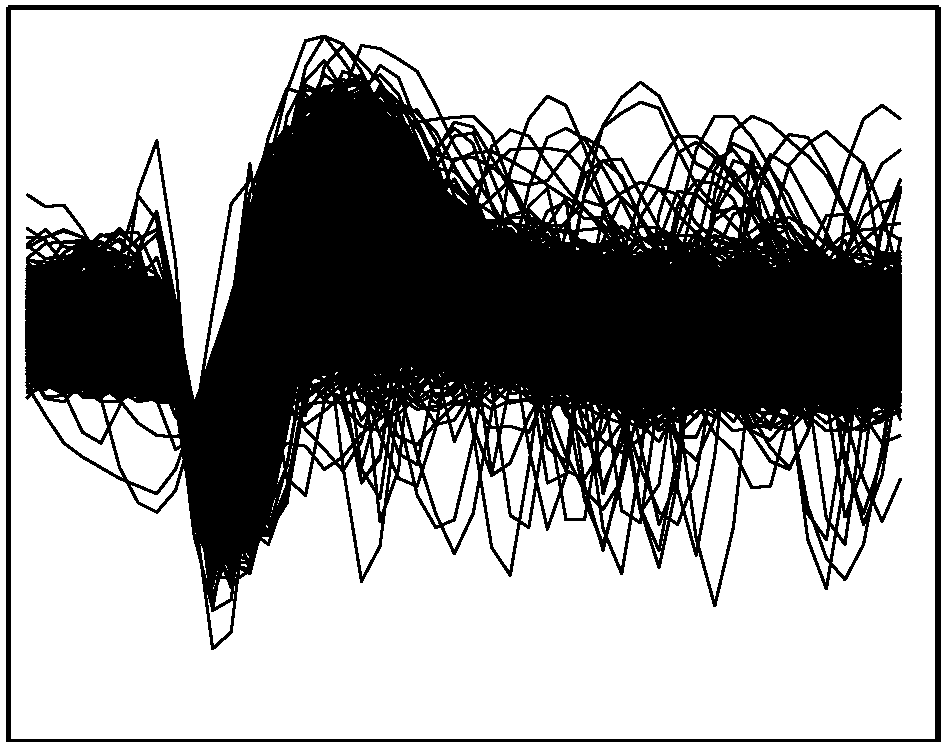
\includegraphics[width=80mm]{figures/waveforms}
\caption{Single channel, all detected action potentials.}
\end{figure}
\end{center}
}

\only<5>{
\begin{center}
\begin{figure}
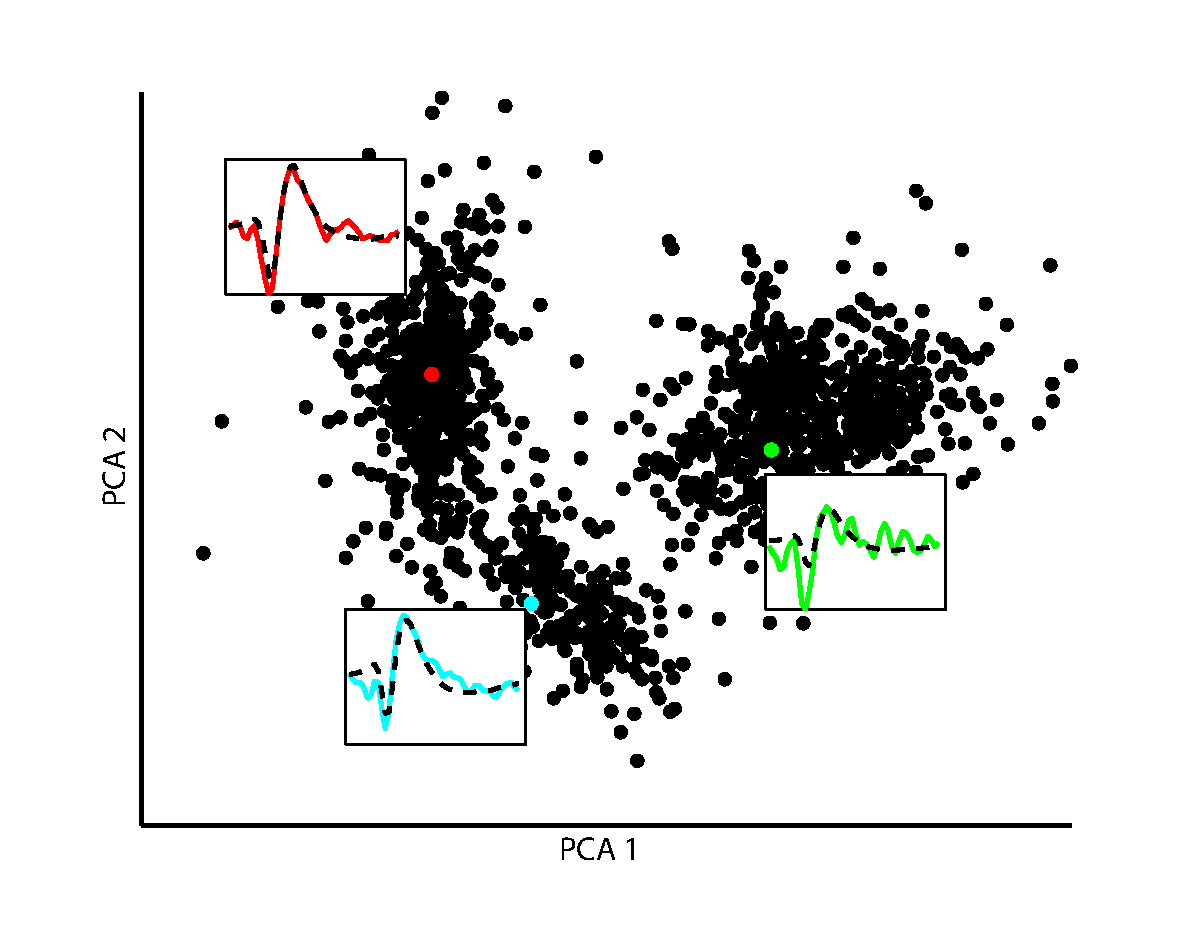
\includegraphics[width=80mm]{figures/pca_projection.pdf}
\caption{Projection of waveforms onto first 2 PCA basis vectors.}
\end{figure}
\end{center}
}
\only<6>{
\begin{center}
\begin{figure}
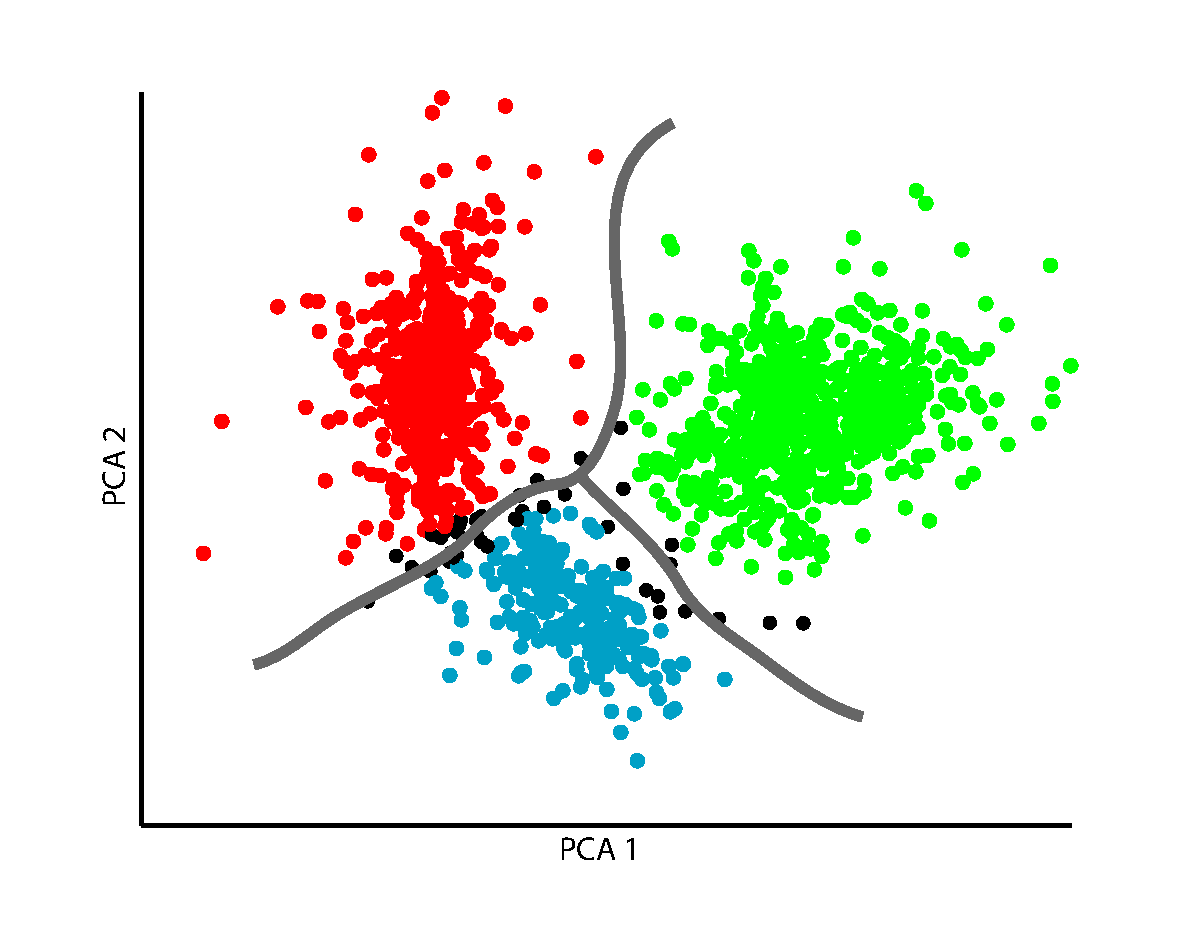
\includegraphics[width=80mm]{figures/pca_projection_sorted.pdf}
\caption{Spike train variability arising from clustering ambiguity.}
\end{figure}
\end{center}
}
\end{frame}


\section{Gaussian Mixture Model}
\subsection{Finite Model}
\begin{frame}
\frametitle{ Gaussian Mixture Model (GMM) Spike Sorting \citep{Lewicki1994}}
\begin{columns}[top]
\column{.4\textwidth}
\begin{center}
%		\begin{figure}
		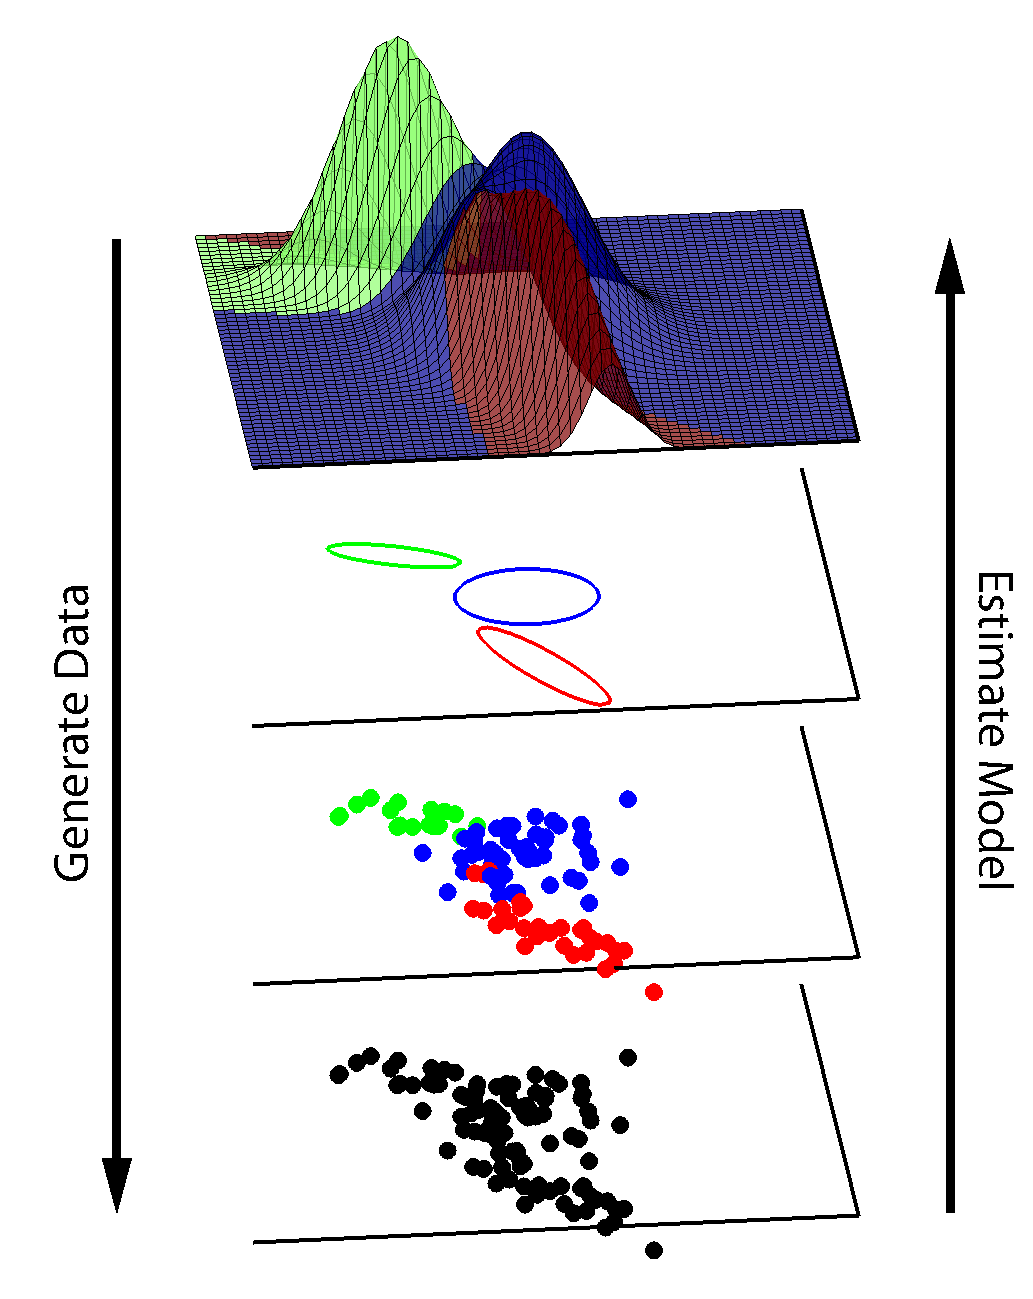
\includegraphics[height=5cm]{figures/generative_model_schematic.pdf}
		%\caption{Generation and estimation.}
%	\end{figure}
\end{center}
\column{.5\textwidth}
\begin{block}{GMM}
{\tiny
\begin{eqnarray*}
\theta_k &=& \{\vec \mu_k,\Sigma_k\} \\
c_i | \vec \pi &\sim& \mbox{Discrete}(\pi_1, \ldots, \pi_K) \\
\vec y_i | c_i=k, \Theta &\sim& \mbox{Gaussian}(\theta_k) \\
\end{eqnarray*}
}
\end{block}
%\begin{block}{Finite Mixture Modeling}
%\begin{itemize}
%\item Latent variable model
%\item One latent cause per observation
%\item Unknown number of latent causes
%\end{itemize}
%\end{block}
\end{columns}
\end{frame}


\begin{frame}
\frametitle{ Finite Gaussian mixture model estimation}
\begin{block}{Estimation}
\begin{itemize}
\item Expectation Maximization (EM)
\item Variational inference
\item Markov chain Monte Carlo (MCMC)
\end{itemize}
\end{block}
\begin{block}{A challenge to pick the ``best'' model}
\begin{itemize}
\item Complexity $\leftrightarrows$ Model selection $\leftrightarrows$ Neuron cardinality
\item Clustering $\leftrightarrows$ Attributing spikes to neurons
\end{itemize}
\end{block}
\begin{block}{Approaches}
\begin{itemize}
\item Reversible jump MCMC
\item Penalized likelihood (Bayesian information criteria)
\item Cross validation on held out data
\item or...
\end{itemize}
\end{block}
\end{frame}
\subsection{Infinite Model}

\section{Infinite GMM}


\begin{frame}
\frametitle{Bayesian GMM $\rightarrow$ IGMM as $K \rightarrow \infty$ \citep{Rasmussen2000}}
\begin{columns}[t]
\column{.2\textwidth}
\begin{center}
\begin{figure}
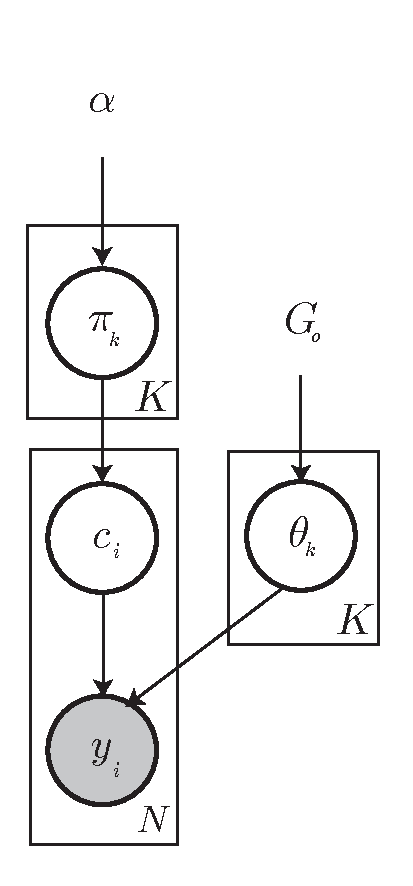
\includegraphics[height=3.75cm]{figures/bgmm_graphical_model.pdf}
\end{figure}
\end{center}
\column{.7\textwidth}
{\tiny
\begin{eqnarray*}
 \Sigma_k &\sim& \mbox{Inverse-Wishart}_{\upsilon_0}( \Lambda_0^{-1}) \\ 
\vec \mu_k &\sim& \mbox{Gaussian}(\vec \mu_0,  \Sigma_k/\kappa_0)
\end{eqnarray*}
\[\theta_k = \{\vec \mu_k,\Sigma_k\}\]
\begin{eqnarray*}
\pi_1, \ldots, \pi_K | \alpha &\sim& \mbox{Dirichlet}(\frac{\alpha}{K}, \ldots, \frac{\alpha}{K}) \\
c_i | \vec \pi &\sim& \mbox{Discrete}(\pi_1, \ldots, \pi_K) \\
\vec y_i | c_i=k, \Theta &\sim& \mbox{Gaussian}(\theta_k) \\
\Theta &\sim& \mathcal{G}_0 \\
\end{eqnarray*}
}
\end{columns}
\begin{block}{Key insight}
IGMM posterior distribution consists of infinite mixture models that vary in realized complexity
\end{block}
{\footnotesize

}
\end{frame}

\begin{frame}
\frametitle{Key insight}
%\begin{block}{Learn multiple models and average}
\begin{center}
\begin{figure}
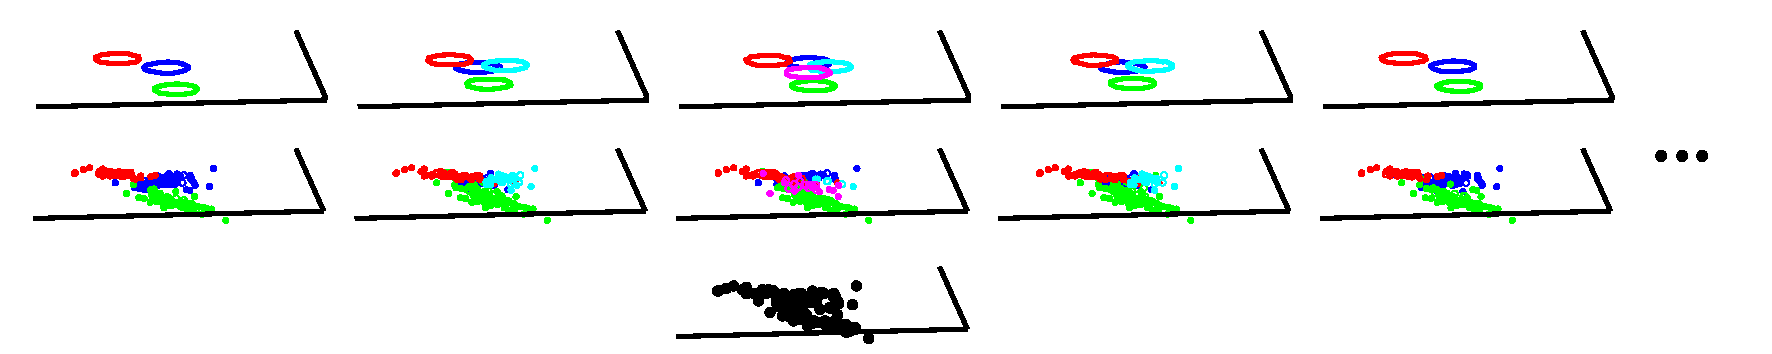
\includegraphics[width=11cm]{figures/posterior_schematic.pdf}
\caption{Multiple generative models for same data.}
\end{figure}
\end{center} 
%\end{block}
%\begin{block}{Bayesian modeling: complexity and clustering}
%As in \cite{nguyenb03} (RJMCMC) and \cite{woodb06} (NPB) one can learn a (posterior) distribution over models that vary in (realized) complexity rather than a single best model.
%\end{block}
\end{frame}



\begin{frame}[t]
\frametitle{IGMM Posterior Estimation}
\begin{block}{Many approaches from DP mixture model literature}
\begin{itemize}
\item Batch: 
\begin{itemize}
\item Markov chain Monte Carlo (MCMC)
\begin{itemize}
\item Gibbs \citep{Neal2000,Maceachern1998}
\item Split merge \citep{Jain2004}
\end{itemize}
\item Variational \citep{Blei2005}
\end{itemize}
\item Sequential: Particle filter \citep{Maceachern1999,Fearnhead2004}
\end{itemize}
\end{block}
\end{frame}




\begin{frame}
\frametitle{IGMM $\approx$ Bayesian GMM in $K \rightarrow \infty$ limit}
\begin{columns}[t]
\column{.2\textwidth}
\begin{center}
\begin{figure}
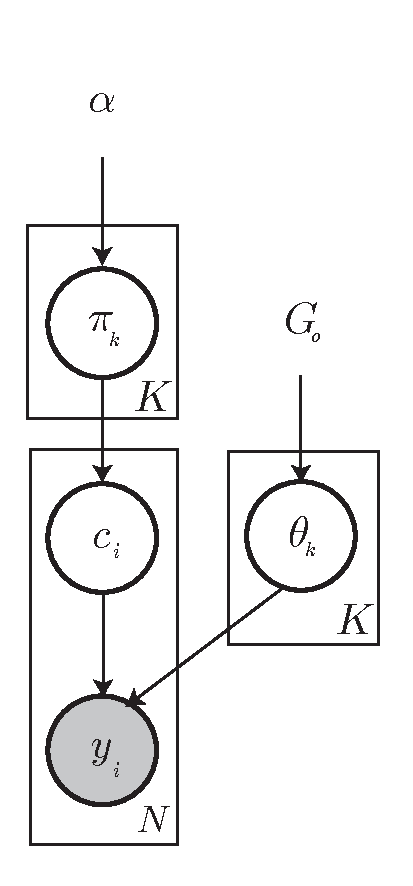
\includegraphics[height=3.75cm]{figures/bgmm_graphical_model.pdf}
\end{figure}
\end{center}
\column{.7\textwidth}
{\tiny
\begin{eqnarray*}
 \Sigma_k &\sim& \mbox{Inverse-Wishart}_{\upsilon_0}( \Lambda_0^{-1}) \\ 
\vec \mu_k &\sim& \mbox{Gaussian}(\vec \mu_0,  \Sigma_k/\kappa_0)
\end{eqnarray*}
\[\theta_k = \{\vec \mu_k,\Sigma_k\}\]
\begin{eqnarray*}
\pi_1, \ldots, \pi_K | \alpha &\sim& \mbox{Dirichlet}(\frac{\alpha}{K}, \ldots, \frac{\alpha}{K}) \\
c_i | \vec \pi &\sim& \mbox{Discrete}(\pi_1, \ldots, \pi_K) \\
\vec y_i | c_i=k, \Theta &\sim& \mbox{Gaussian}(\theta_k) \\
\Theta &\sim& \mathcal{G}_0 \\
\end{eqnarray*}
}
\end{columns}

\end{frame}



\subsection{Conjugacy}
\begin{frame}[t]
\frametitle{Dirichlet Multinomial Conjugacy}
\begin{eqnarray*}
\vec{\pi} & \sim & \text{Dir}\left(\frac{\alpha}{K},\ldots,\frac{\alpha}{K}\right) \\
P(c_{i+1} = k|c_1,\ldots,c_{i},\alpha) & = & \int P(c_{i+1} = k | \vec{\pi}) p(\vec{\pi}|c_1,\ldots,c_{i},\alpha) d\vec{\pi} \\
= \frac{\Gamma(\alpha + i )}{\prod_{j=1}^{K}\Gamma(\frac{\alpha}{K} + n_j)} &&\int\pi_1^{\frac{\alpha}{K}+n_1 -1}\ldots\pi_k^{\frac{\alpha}{K}+n_k}\ldots\pi_K^{\frac{\alpha}{K}+n_K-1}d\vec{\pi} \\
& = & \frac{n_k + \frac{\alpha}{K}}{\alpha + i}
\end{eqnarray*}
Where $n_k$ is the number of $c_j$, $j = 1,\ldots,i$ such that $c_j = k$.   
\newline

Note that this is true regardless of the ``order'' of the observations ($c_i$'s form an exchangeable sequence).
\end{frame}

\subsection{Taking the Infinite Limit}

\begin{frame}[t]
\frametitle{Chinese Restaurant Process}

Order the clusters so $n_k > 0$ if $k \le K_+$ and $n_k = 0$ if $k > K_+$.  Then as $K\rightarrow\infty$

\begin{equation*}
P(c_{i+1} = k | c_1,\ldots,c_{i},\alpha) = 
\left\{ \begin{array}{l} 
       \frac{n_k}{\alpha+i} \quad k \leq K_+\\ 
	\frac{\alpha}{\alpha+i} \quad k>K_+ \end{array} \right..
\label{eqn:crp}
\end{equation*}
This is the {\em Chinese Restaurant Process}, $CRP(\alpha)$.
\end{frame}


\begin{frame}[t]
\frametitle{Fully Conjugate Collapsed IGMM Gibbs Sampler}
One can make a ``collapsed'' Gibbs sampler for the IGMM by analytically integrating out the $\pi$'s and $\theta$'s leaving on the $c$'s to sample.  The Gibbs sampler will be constructed by finding the posterior distribution of a single $c$ conditioned on the state of all other variables, then sampling each of these variables repeatedly.
\begin{block}{Gibbs sampler for the IGMM}
\begin{eqnarray}
P(c_i = j | \mathcal{C}_{-i}, \mathcal{Y}, \alpha; \mathcal{H}) &\propto& P(\mathcal{Y} | \mathcal{C}; \mathcal{H}) P(\mathcal{C}|\alpha) \nonumber \\
%&\propto& \prod_{j=1}^{K_+} P(\mathcal{Y}^{(j)}; \mathcal{H}) P(c_i = j | \mathcal{C}_{-i}, \alpha) \nonumber \\
%&\propto& P(\mathcal{Y}^{(j)}; \mathcal{H}) P(c_i = j |  \mathcal{C}_{-i}, \alpha)\nonumber \\ 
&\propto& P(y_i | \mathcal{Y}^{(j)} \backslash y_i; \mathcal{H}) P(c_i = j |  \mathcal{C}_{-i}, \alpha) \nonumber
\label{eqn:clpsed_gibbs_cid_conditional}
\end{eqnarray}
\end{block}
\end{frame}

\begin{frame}
\frametitle{Fully Conjugate Collapsed IGMM Gibbs Sampler}
\begin{block}{Per class posterior predictive distribution}
\begin{equation} y_i | \mathcal{Y}^{(j)} \backslash y_i; \mathcal{H} \sim t_{\nu_n-D+1}(\vec \mu_n, {\bf \Lambda}_n(\kappa_n +1) / (\kappa_n(\nu_n-D+1)))
\label{existing_table_posterior_predictive}
\end{equation}

\noindent where 

\begin{eqnarray*}
\vec \mu_n &=& \frac{\kappa_0}{\kappa_0+N}\vec \mu_0 + \frac{N}{\kappa_0+N}\bar y \\
\kappa_n &=& \kappa_0+N \\
\nu_n &=& \nu_0 + N \\
{\bf \Lambda}_n &=& {\bf \Lambda}_0 + {\bf S} + \frac{\kappa_0n}{\kappa_0+N}(\bar y - \vec \mu_0)(\bar y - \vec \mu_0)^T
\end{eqnarray*}
\end{block}
\end{frame}

\section{Results}

\begin{frame}
\frametitle{Microelectrode Array Data {\tiny la040325MI}}
\only<1>{
\begin{center}
\begin{figure}
\begin{tabular}{c|c}
		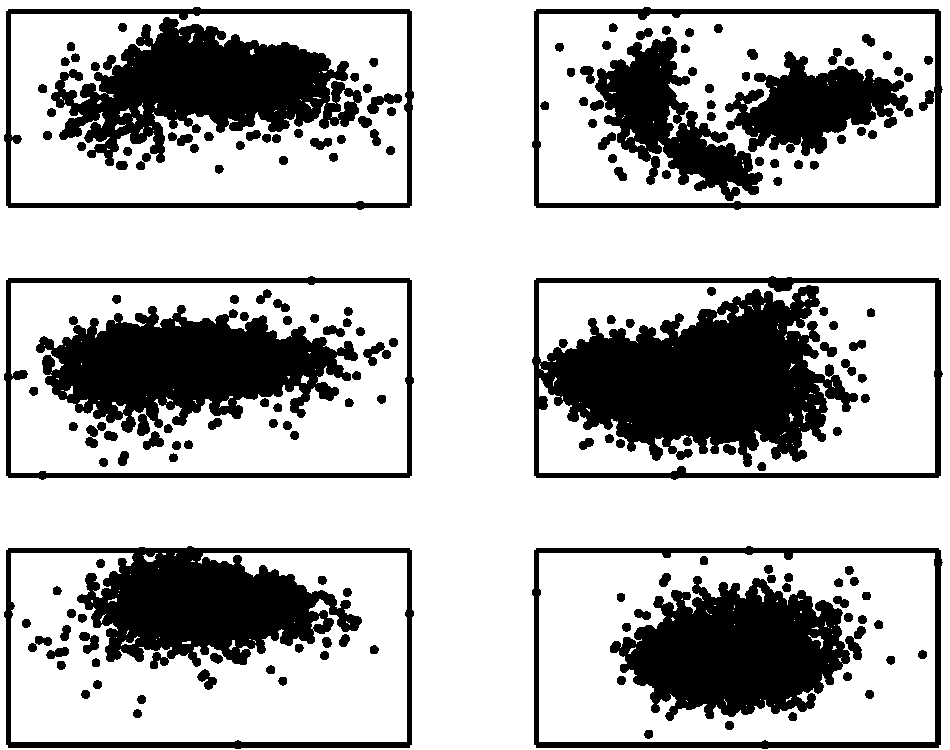
\includegraphics[width=50mm]{figures/la040324mi_unsorted_array_data} &
	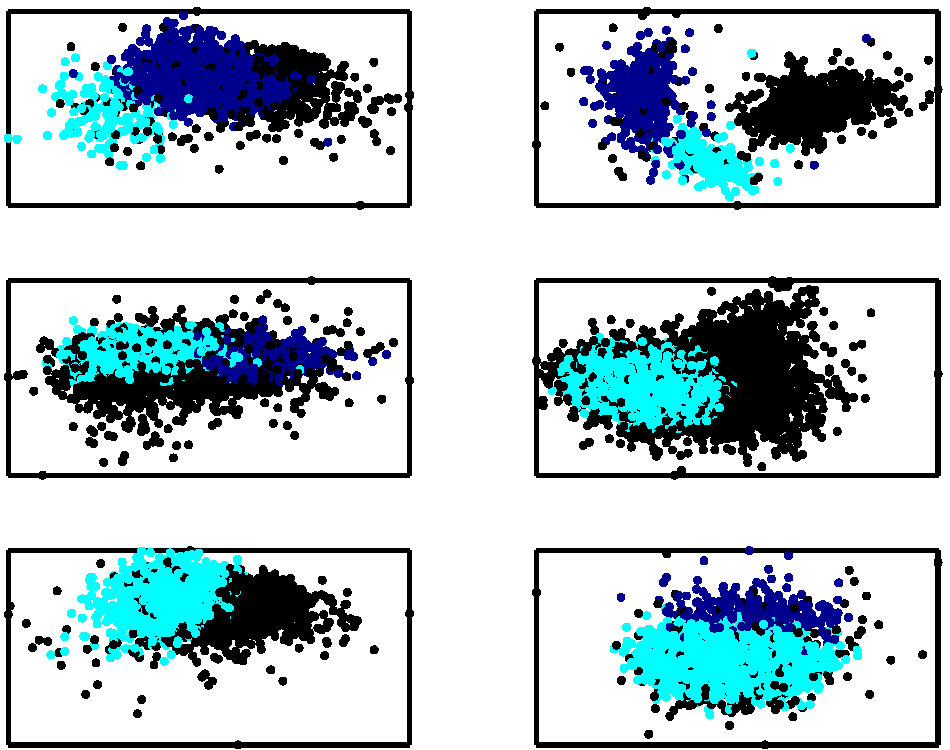
\includegraphics[width=50mm]{figures/la040324mi_human_sorted_array_data}
	\end{tabular}
	\caption{Unsorted \& Human Sorted}
\end{figure}
\end{center}
}
\only<2>{
\begin{center}
\begin{figure}
\begin{tabular}{c|c}
		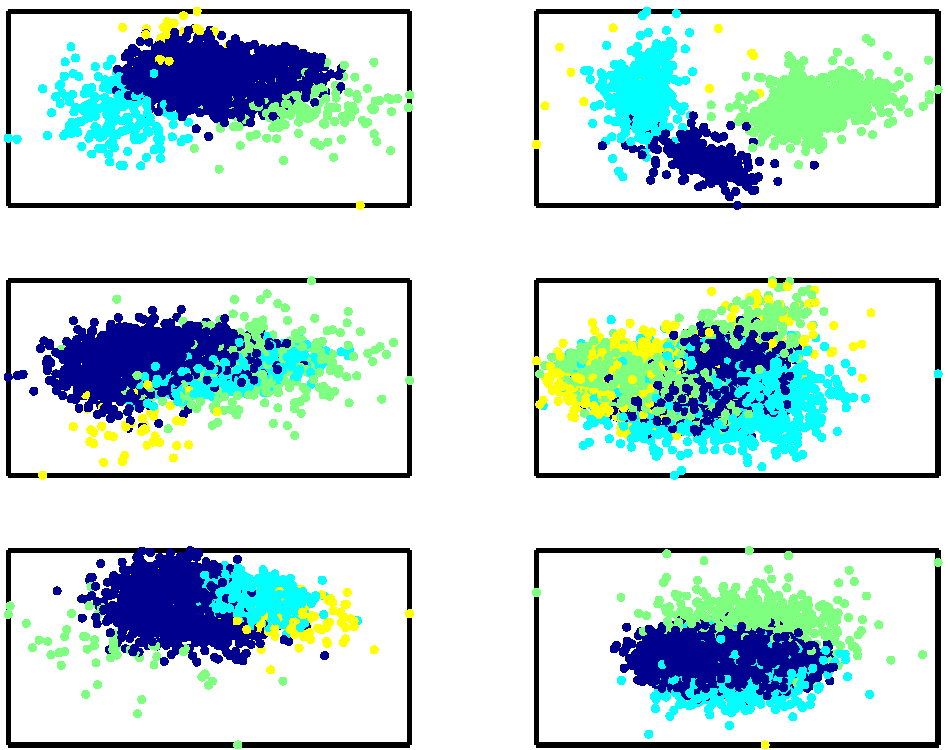
\includegraphics[width=50mm]{figures/la040324mi_gibbs_sample_1250_array_data} &
	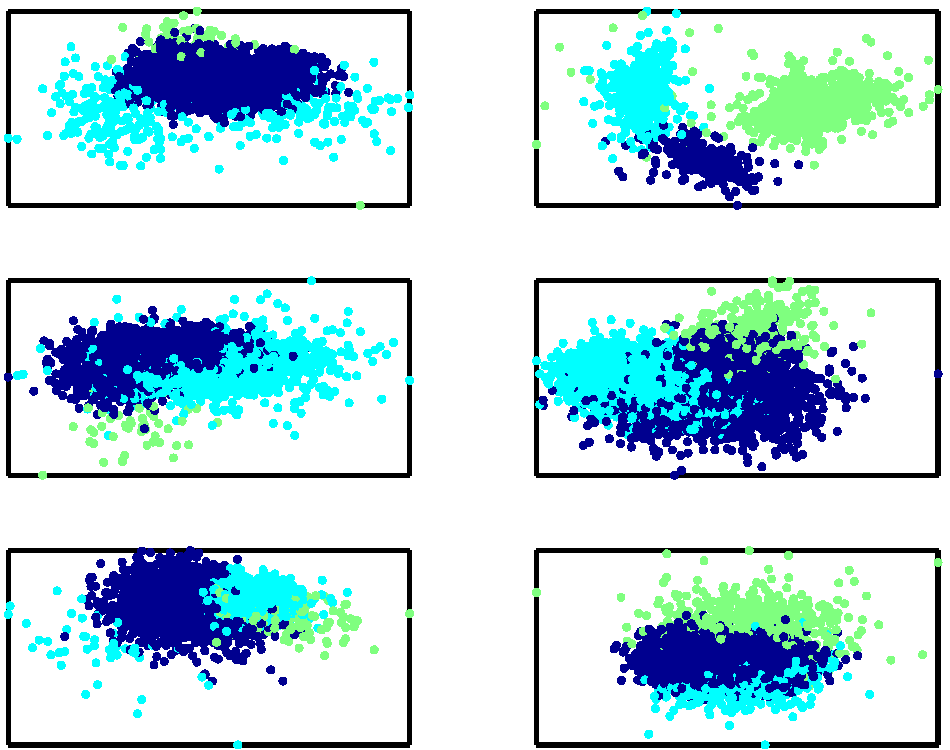
\includegraphics[width=50mm]{figures/la040324mi_gibbs_sample_1500_array_data}
	\end{tabular}
	\caption{ IGMM }
\end{figure}
\end{center}
}
%\only<4>{
%\begin{center}
%\begin{figure}
%\begin{tabular}{c|c}
%		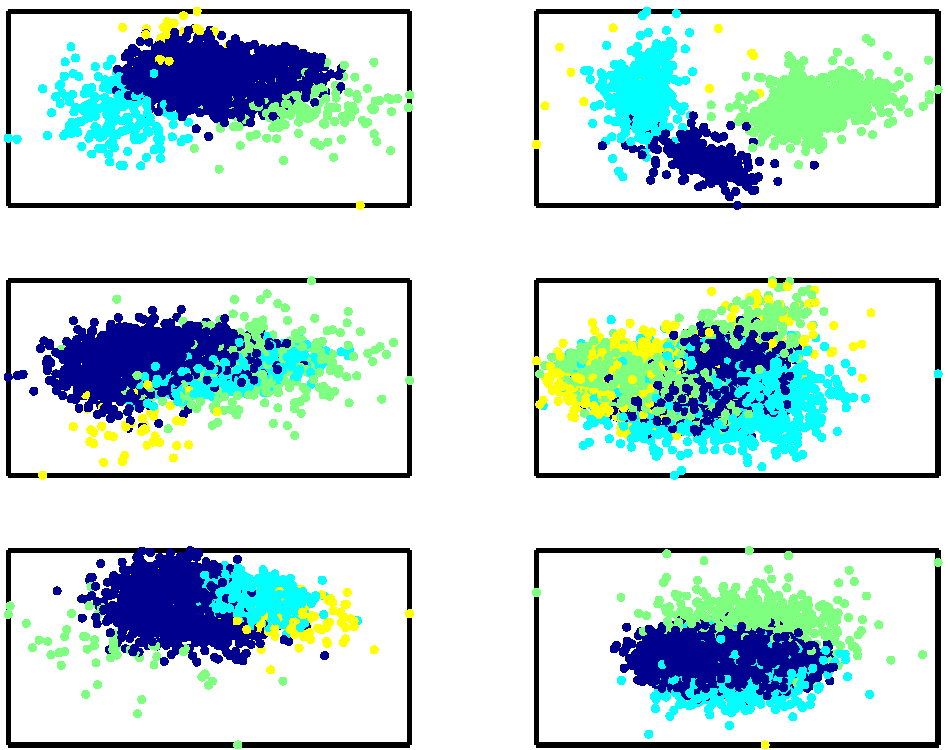
\includegraphics[width=50mm]{figures/la040324mi_gibbs_sample_1250_array_data} &
%	\includegraphics[width=50mm]{figures/la040324mi_gibbs_sample_1500_array_data_highlighted}
%	\end{tabular}
%	\caption{ IGMM }
%\end{figure}
%\end{center}
%}
\only<3>{
\begin{center}
\begin{figure}
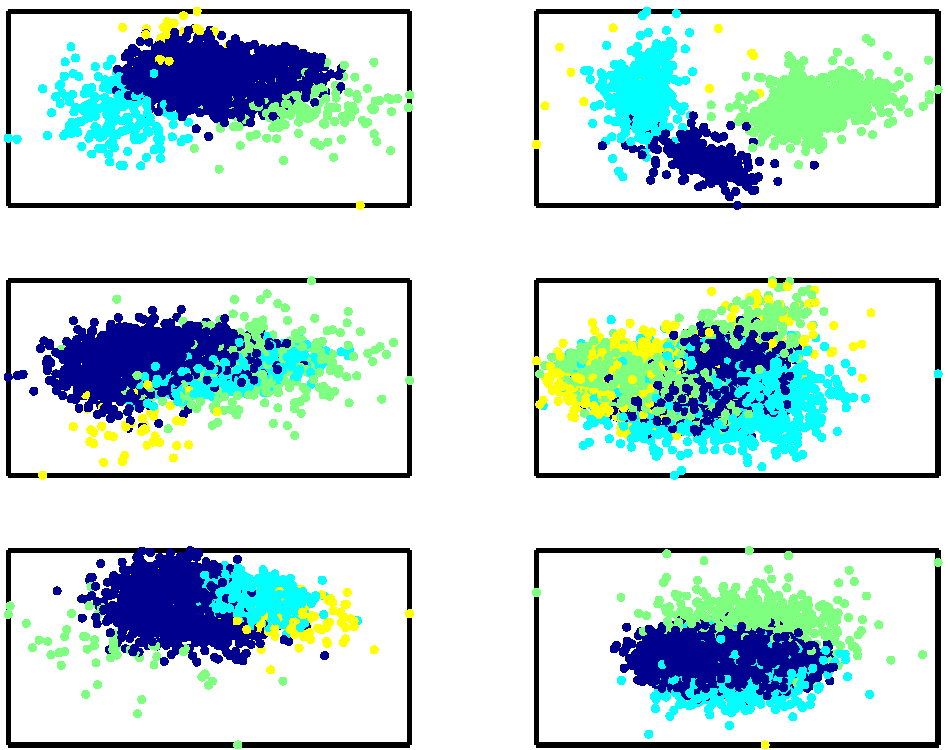
\includegraphics[width=70mm]{figures/la040324mi_gibbs_sample_1250_array_data}
\end{figure}
\end{center}
}
\only<4>{
\begin{center}
\begin{figure}
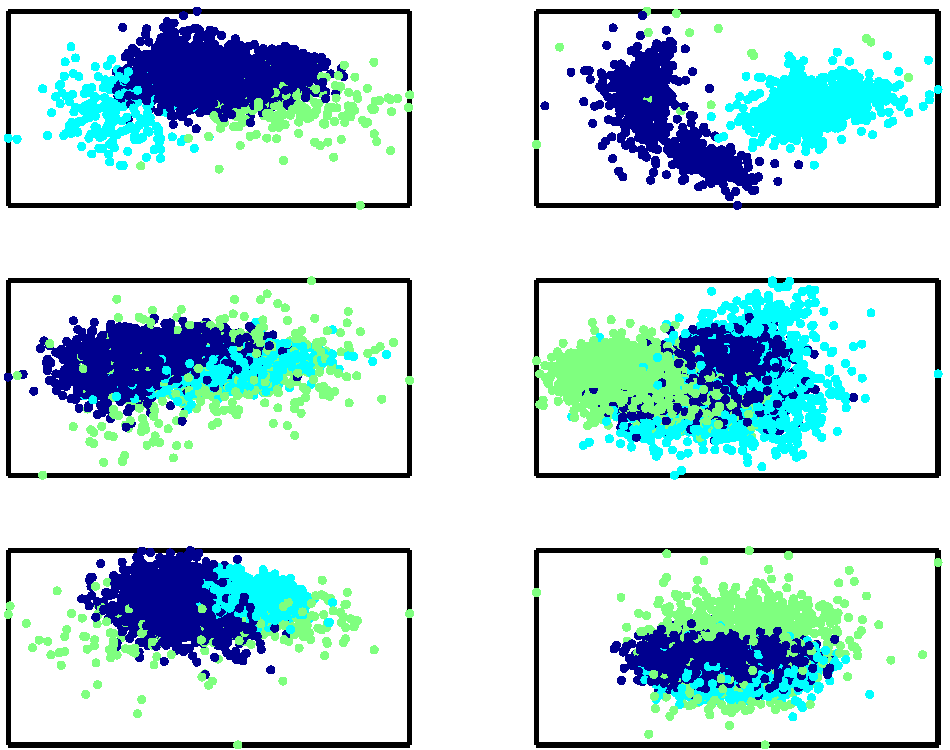
\includegraphics[width=70mm]{figures/la040324mi_gibbs_sample_1000_array_data}
\end{figure}
\end{center}
}
\only<5>{
\begin{center}
\begin{figure}
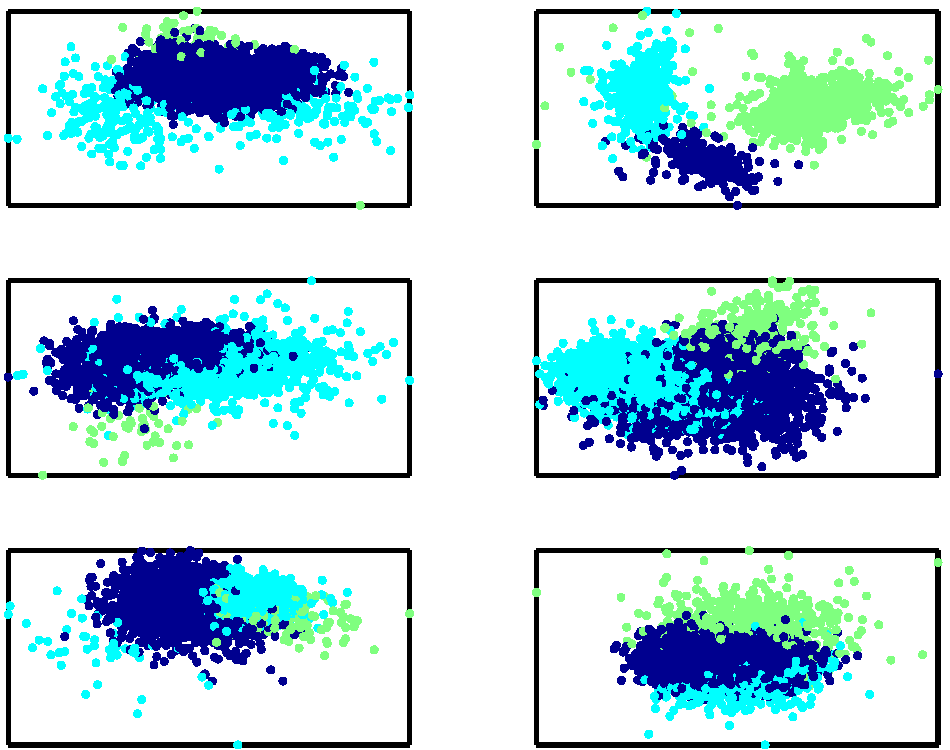
\includegraphics[width=70mm]{figures/la040324mi_gibbs_sample_1500_array_data}
\end{figure}
\end{center}
}
\only<6>{
\begin{center}
\begin{figure}
\begin{tabular}{c|c}
		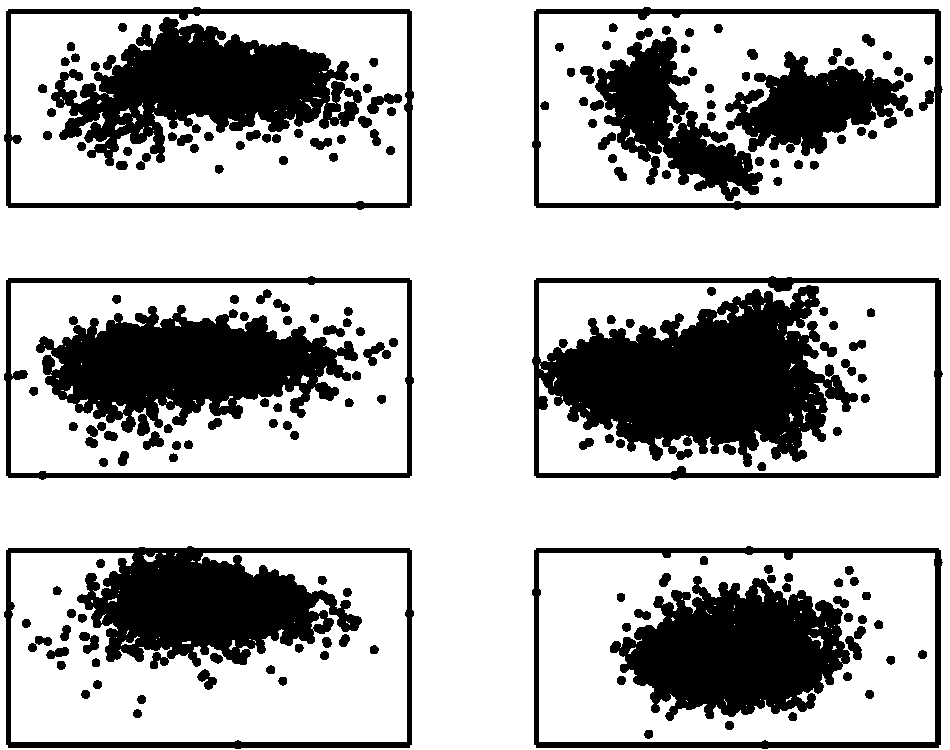
\includegraphics[width=50mm]{figures/la040324mi_unsorted_array_data} &
	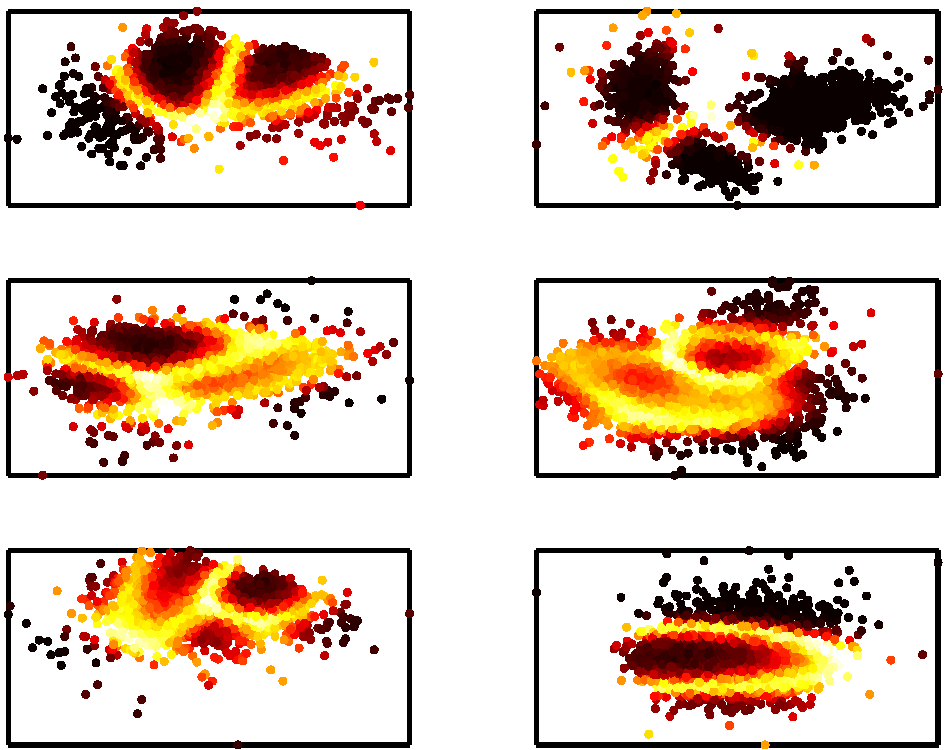
\includegraphics[width=50mm]{figures/la040324mi_ambiguity_array_data}
	\end{tabular}
	\caption{ Unsorted \& Ambiguity }
\end{figure}
\end{center}
}
\end{frame}



\bibliographystyle{plainnat}
\begin{frame}[allowframebreaks]
\frametitle{Bibliography}
\bibliography{../../papers/uber} 
\end{frame}
\end{document}